\subsection{Aufbau der Schaltung}
Das Mikrocontroller-System, welches für das Aufnehmen und Übertragen der Messdaten zuständig ist, besteht im Wesentlichen aus vier Bestandteilen, die miteinander verbunden sind:
\begin{enumerate}
\item Dem \textbf{Grove EMG-Sensor} \cite{Src:EMGdetect}~, der per Elektromyografie Messungen über die Stärke der Armmuskel-Kontraktionen erhebt. Dabei wird die elektrische Muskelaktivität anhand von Potentialänderungen auf der Haut mithilfe von drei Oberflächenelektroden gemessen. Diese Signale werden durch den Sensor verstärkt und gefiltert. Zuletzt gibt dieser eine Spannung im Bereich von 1,5 bis 3,3 Volt aus, wobei eine höhere Spannung höhere Muskelaktivität bedeutet. Dabei wird eine Versorgungsspannung von 3,3 bis 5 Volt benötigt.
\item Dem Mikrocontroller \textbf{Atmel ATmega 88PA} \cite{Src:AtmelDBeins}~, welcher die vom EMG-Sensor gelieferten Daten an den Bluetooth-Chip weitergibt. Es handelt sich hierbei um einen 8-Bit-Mikrocontroller\cite{Src:AtmelDBzwei}~, d.h. es können pro Takt maximal 8 Bit verarbeitet werden. Dieser folgt der sogenannten RISC-Architektur, welche einen reduzierten Befehlssatz im Vergleich zu Standardcomputern besitzt, dafür aber schneller arbeitet. Damit eignet er sich gut für den beabsichtigten Einsatzzweck, bei dem Daten möglichst schnell auf das Mobilgerät übertragen werden sollen. \\
Weiterhin setzt dieser Controllertyp die Harvard-Struktur um. \cite{Src:SchmittAVR} Es existieren also getrennte Speicher- und Adressbereiche für Befehle und Daten. Die peripheren Schnittstellen können über Portadressen angesprochen werden. Zu diesen Schnittstellen zählen zwei für die beabsichtigte Anwendung nötige, denn es werden sowohl eine UART-Schnittstelle zur Kommunikation mit dem Bluetooth-Chip als auch ein Analog-Digital-Wandler zum Einlesen der Ausgangsspannung des EMG-Sensors angeboten. Das Programm kann bei diesem Controller über ein Entwicklungsgerät in den Programmspeicher (Flash) geladen werden.
\item Dem Bluetooth-Chip \textbf{HC-05} \cite{Src:BluetoothHC}~, welcher eine Möglichkeit zur drahtlosen Kommunikation mit dem Android-Mobilgerät über Funk nach dem Bluetooth-Standard bereitstellt. Dabei sind alle zur Kommunikation nötigen Bestandteile auf einem Chip integriert. Der HC-05 wird über die UART-Schnittstelle (Universal Asynchronous Receiver Transmitter) angesprochen, wobei diese eine digitale serielle Schnittstelle zur Datenübertragung realisiert. Der Bluetooth-Chip kommuniziert standardmäßig mit 9600 Baud.
\item Einem \textbf{Quarzoszillatoren} mit eingebautem Schwingquarz, in diesem Fall mit der Frequenz 8 MHz, welcher einen genauen Systemtakt für den Mikrocontroller liefert. Dieser wird benötigt, um eine möglichst störungsfreie UART-Kommunikation realisieren zu können. Der Oszillator muss in den Einstellungen (Fuses) des Mikrocontrollers als Taktquelle ausgewählt (\texttt{CKSEL}-Bit) und die interne Teilung des Taktes durch 8 abgeschaltet (\texttt{CKDIV8}-Bit) werden.
\end{enumerate}
Diese Bestandteile wurden nach dem auf der folgenden Seite sichtbaren Schaltplan (\autoref{fig:mikrocontroller}) verbunden.
\subsection{Entwicklung des Programms auf dem Mikrocontroller}
Das Programm (siehe \autoref{listing:mikrocontroller}, S. \pageref{listing:mikrocontroller}) wurde in der Programmiersprache C geschrieben und besteht aus sechs Funktionen, die jedoch auf einige in den C-Standardbibliotheken vorhandene Funktionen und Definitionen für den C-Präprozessor zurückgreifen. Zusätzlich tätigt das Programm auch einige eigene Definitionen für den Präprozessor. Alle Funktionen außer der Main-Funktion, mit der das Programm startet, werden dem Compiler zunächst als Funktionsprototypen mithilfe ihrer Signaturen bekanntgemacht und erst nach der Main-Funktion definiert. Im einzelnen sind folgende Funktionen definiert:
\begin{itemize}
\item \texttt{init()}. Diese Funktion initialisiert die einzelnen Funktionen des Controllers, indem sie die entsprechenden Einstellungsregister \cite{Src:AtmelDBeins} setzt. Der Analog-Digital-Wandler wird aktiviert und dessen interner Taktteiler gesetzt. Die Sende- und die Empfangsfunktion der UART-Schnittstelle werden ebenfalls aktiviert und deren Baudratenfaktor, der angibt, wie schnell kommuniziert werden soll, gesetzt.
Der Baudratenfaktor \cite{Src:AtmelDBeins} berechnet sich aus (gerundet): \[UBBR = \frac{f_{CPU}}{16 \cdot r_{BAUD}} - 1 \]
Anschließend werden beide Schnittstellen zum ersten Mal ausgelesen, um ihre Funktionsfähigkeit sicherzustellen.
\item \texttt{u\_putch()}. Hier werden einzelne Zeichen (\textit{Char}) über die UART-Verbindung übertragen. Dabei muss gewartet werden, bis diese Verbindung freigegeben wird.
\item \texttt{u\_puts()}. Diese Funktion überträgt Zeichenketten (\textit{String}) über UART. Hierzu wird über die einzelnen Zeichen mithilfe der in C integrierten Zeigerarithmetik iteriert und jeweils \texttt{u\_putch()} aufgerufen.
\item \texttt{delay()} lässt den Mikrocontroller für die angegebene Zahl an Sekunden warten. Dazu wird die in der Bibliothek \texttt{util/delay.h} definierte Funktion \texttt{\_delay\_ms()} benutzt.
\item \texttt{sendCurrentVoltage()}. In dieser Funktion wird eine Analog-Digital-Wandlung gestartet und nach deren Abschluss das Ergebnis ausgelesen. Dabei handelt es sich um einen relativen Wert im Vergleich zur Referenzspannung \cite{Src:AVRTutor}, weshalb die eigentliche Spannung aus der Gleichung $U = \frac{x}{1024} \cdot U_{ref}$ gewonnen wird.\footnote{Hierbei ergibt sich jedoch insoweit ein Problem, als dass die Versorgungsspannung bei Batteriebetrieb schwanken kann.} Die dabei entstandene Gleitkommazahl wird mithilfe der Bibliotheksfunktion \texttt{sprintf()} in einen String geschrieben, der per \texttt{u\_puts()} übertragen werden kann.
\item \texttt{main()}. In dieser Funktion wird zuerst \texttt{init()} aufgerufen. Anschließend wird in einer Endlosschleife im Abstand einer halben Sekunde \texttt{sendCurrentVoltage()} gestartet und die Spannung an das Mobilgerät übertragen. Es muss sich hier um eine Endlosschleife handeln, da der Mikrocontroller nach der Ausführung von \texttt{main()} in ein undefiniertes Verhalten übergeht, aus dem er nur durch Neustart befreit werden kann.
\end{itemize}
\begin{figure}[H]
\centering
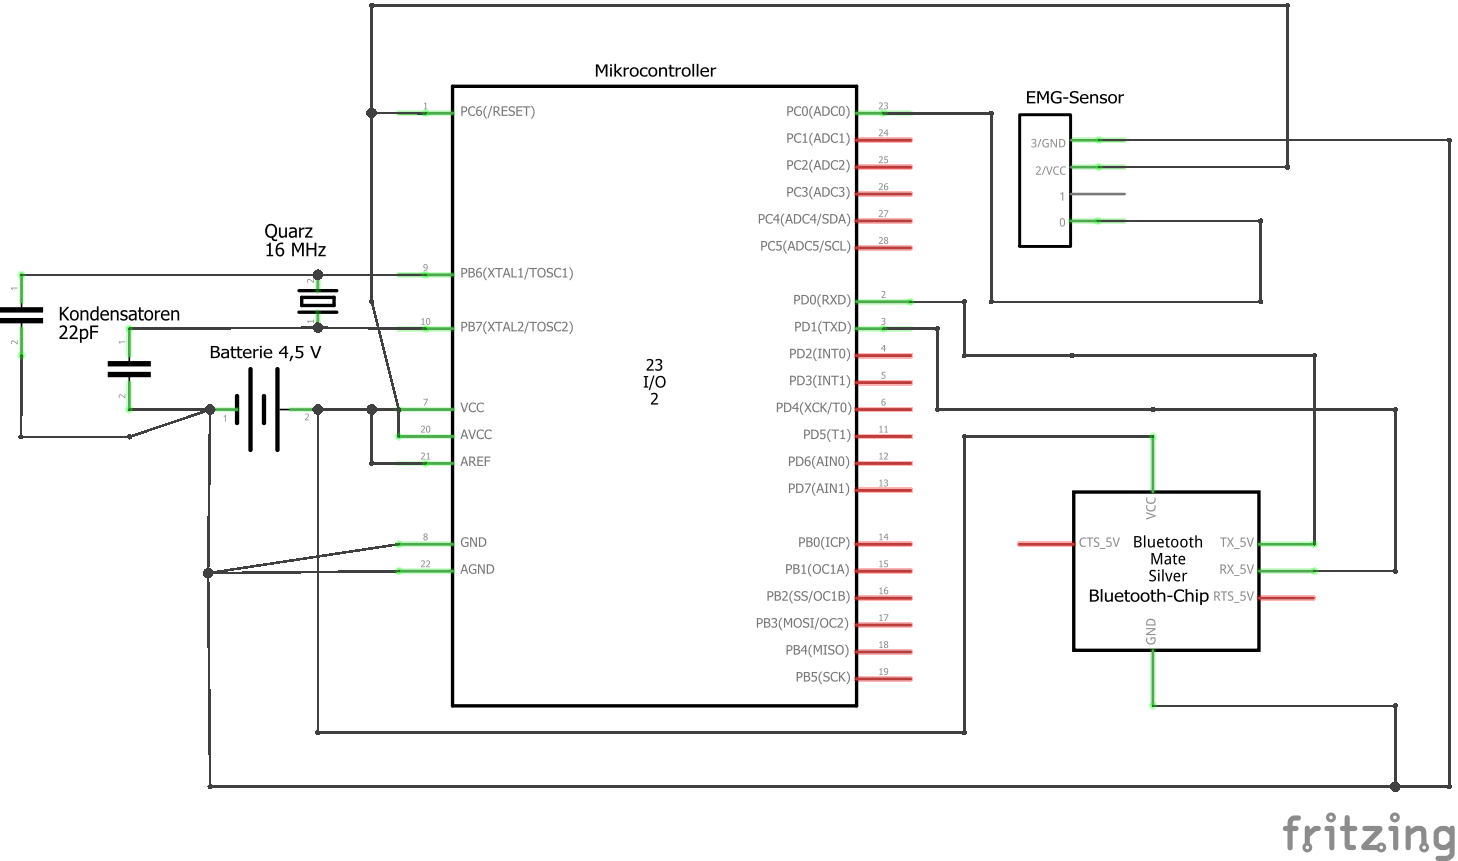
\includegraphics[width=0.8\textwidth]{pics/mikrocontroller_schaltplan.png}
\caption{Der Schaltplan des Mikrocontrollers}
\label{fig:mikrocontroller}
\end{figure}